\documentclass{beamer}
%
% Choose how your presentation looks.
%
% For more themes, color themes and font themes, see:
% http://deic.uab.es/~iblanes/beamer_gallery/index_by_theme.html
%
\mode<presentation>
{
  \usetheme{Madrid}      % or try Darmstadt, Madrid, Warsaw, ...
  \usecolortheme{beaver} % or try albatross, beaver, crane, ...
  \usefonttheme{serif}  % or try serif, structurebold, ...
  \setbeamertemplate{navigation symbols}{}
  \setbeamertemplate{caption}[numbered]
} 

%%% Работа с русским языком
\usepackage{cmap}					% поиск в PDF
\usepackage[T2A]{fontenc}			% кодировка
\usepackage[utf8]{inputenc}			% кодировка исходного текста
\usepackage[english,portuguese, main=russian]{babel}	% локализация и переносы

%Диаграмы
\usepackage{smartdiagram}

\usepackage[english]{babel}
%\usepackage[utf8x]{inputenc}
%\usepackage{xcolor}
\usepackage{listings}
\lstset
{
    language=[LaTeX]TeX,
    breaklines=true,
    basicstyle=\tt\scriptsize,
    %commentstyle=\color{green}
    keywordstyle=\color{blue},
    %stringstyle=\color{black}
    identifierstyle=\color{magenta},
}

\title[Научно-исследовательский семинар]{Обзор статей для комплинг исследования научно-популярных текстов}
\author{Анастасия Кузнецова, Анна Лапидус, \\ Юлия Коломенская, Ксения Самойленко}
\institute{НИУ ВШЭ}
\date{24 января 2017}

\AtBeginSection[]
{
  \begin{frame}<beamer>
    \frametitle{План доклада}
    \tableofcontents[currentsection,currentsubsection]
  \end{frame}
}

\begin{document}

\begin{frame}
  \titlepage
\end{frame}

% Uncomment these lines for an automatically generated outline.
\begin{frame}{План}
  \tableofcontents
\end{frame}

\section{Topic Modeling}
\begin{frame}{Topic Modeling}
\textbf{Задача:}
определить тематику документов в коллекции

\begin{itemize}
\item Тема - вероятностное распределение слов
\item Документ - вероятностное распределение тем
\end{itemize}

Latent Diriсhlet alloсation. Blei D. M., Ng A. Y., Jordan M. I.\\ 
Journal of Maсhine Learning Researсh.  2003

\end{frame}
\begin{frame}
\begin{figure}
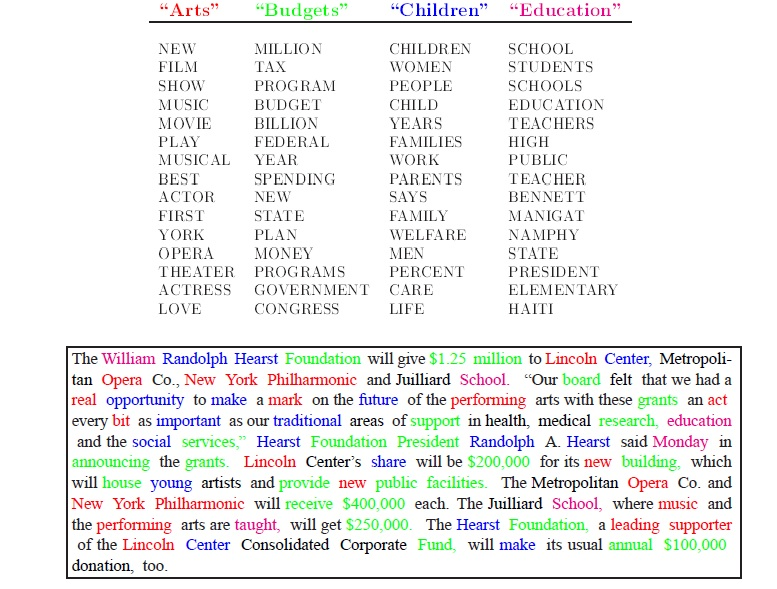
\includegraphics[height=8cm]{topmod1.jpg}
\end{figure}
\end{frame}


\begin{frame}{LDA}

\begin{itemize}
\item Выделяет скрытые темы
\item Определяет частотные тематические слова
\item Bag of Words
\item Темы не когерентны
\end{itemize}

\end{frame}

\begin{frame}{Word Embeddings}
Gaussian LDA for Topic Models with Word Embeddings\\ Rajarshi Das, Manzil Zaheer, Chris Dyer
\begin{itemize}
\item Вместо дискретного распределения на множестве слов - распределение на множестве word embeddings
\item Семантическая связь между тематическими словами
\item Позволяет выделять новые тематические слова
\end{itemize}

\end{frame}
\begin{frame}
\begin{figure}
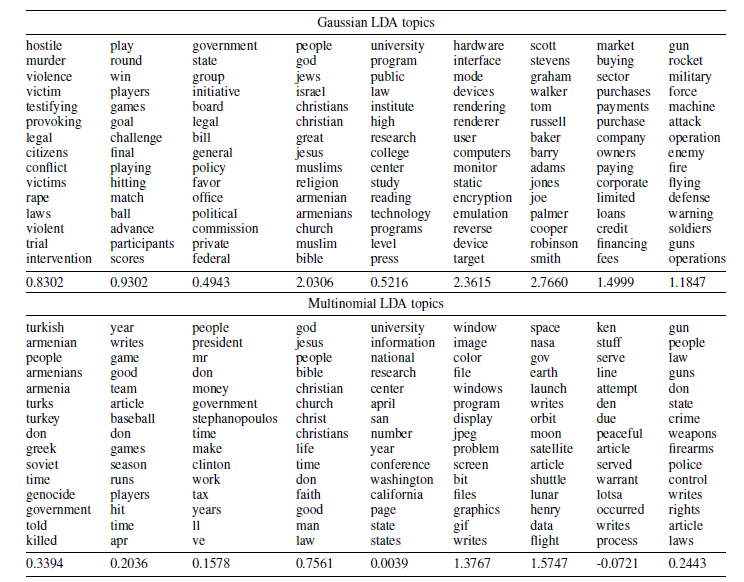
\includegraphics[height=8cm]{topmod2.png}
\end{figure}
\end{frame}

\begin{frame}
\begin{figure}
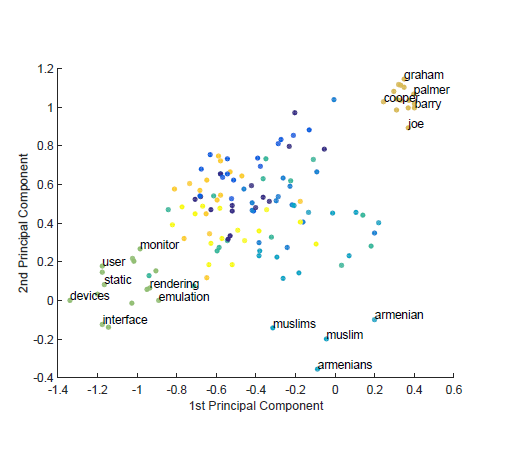
\includegraphics[height=8cm]{topmod3.jpg}
\end{figure}
\end{frame}

\begin{frame}{Другие модели}
\begin{itemize}
\item Мультимодальные тематическое моделирование\\
Tag-weighted topic model for mining semi-structured documents. Li S., Li J., Pan R. 
\item Модель коррелированных тем\\
A correlated topic model of Science. Blei D., Lafferty J. 
\end{itemize}

\end{frame}

\begin{frame}{A correlated topic model of Science. Blei D., Lafferty J.}
\begin{itemize}
\item Логнормальное многомерное распределение позволяет учитывать взаимосвязь между темами
\item Построен граф тематик статей журнала Science
\item На основе верятностых мер (расстояние Хеллингера) определяются наиболее близкие статьи
\end{itemize}

\end{frame}

\begin{frame}
\begin{figure}
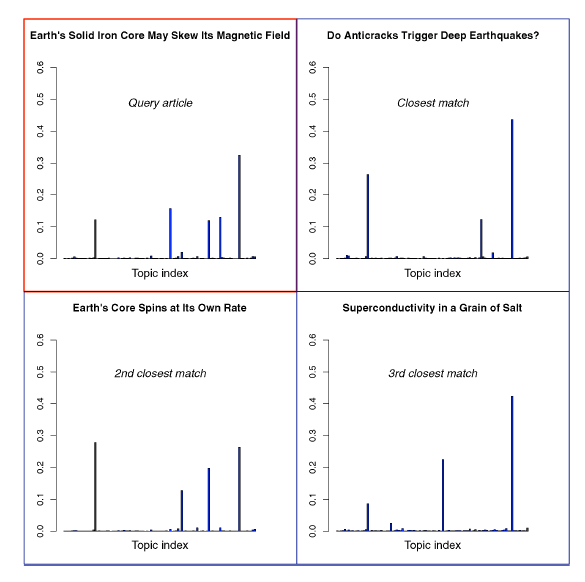
\includegraphics[height=8cm]{topmod4.jpg}
\end{figure}
\end{frame}

\begin{frame}
\begin{figure}
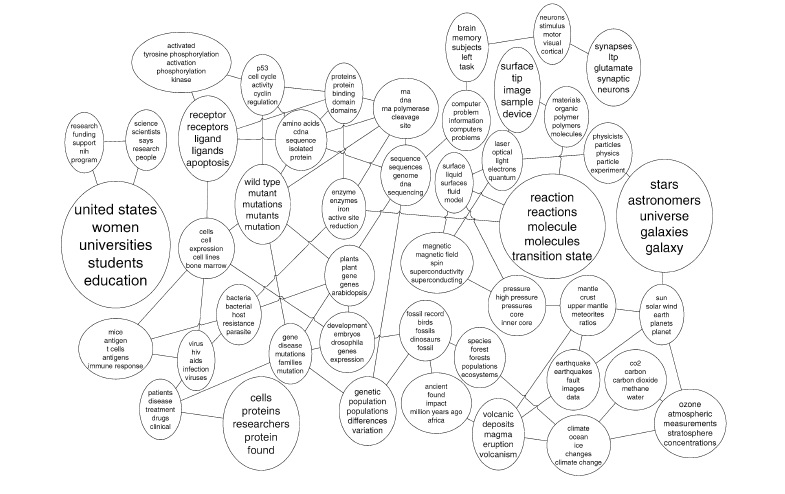
\includegraphics[height=8cm]{topmod5.jpg}
\end{figure}
\end{frame}


\section{Term extraction}
\begin{frame}{Term Extraction}
Term extraction (recognition, identification, acquisition) - преследует различные цели:
\begin{itemize}
\item cоздание онтологии;
\item создание глоссария;
\item составление указателей (indexing)
\item научные исследования и пр.
\end{itemize}


\end{frame}

\begin{frame}{Принцип работы большинства экстракторов:}
\begin{itemize}
\item Предобработка текстов
\item Отбор кандидатов
\item Ранжирование или сортировка кандидатов
\item Валидация (сравнение выбранных показателей с определенным пороговым значением)
\end{itemize}

\end{frame}

\begin{frame}{Лингвистические характеристики термина:}

\begin{itemize}
\item Синтаксическая структура (в основном существительные или именные группы) (для n-грамм) \textit{(нужен POStagger, отбирается слишком много кандидатов -> stop lists)} 
(1) ((Adj|Noun)+|((Adj|Noun)*(NounP rep(Adj|Noun*))Noun
(2) Noun1(Adj|(P rep(Det)?)?Noun2|V Inf)
\item Морфологическая структура (сложносоставные термины, латинские аффиксы)
\item Типичная структура контекстного окружения (определения (vector spaces), пояснения (regexp)) 

\end{itemize}

\end{frame}

\begin{frame}{Статистические характеристики термина:}
\begin{itemize}
\item Частотность
\item Co-occurrence measure (the Dice coefficient, Pointwise Mutual Information (PMI), Log-Likelihood ratio)
\end{itemize}

		\textit{nested terms: floating point arithmetic -> floating point, BUT point arithmetic}

\end{frame}

\begin{frame}{Дистрибутивные характеристики термина:}

			
\begin{itemize}
\item Между словами в n-граммах (unithood)
\end{itemize}
\begin{itemize}
\item Внутри документа или в коллекции документов (termhood, -> tf-idf)
\item Weirdness (specific corpus domain vs general corpus)
\end{itemize}


\end{frame}

\begin{frame}{Оценка работы экстрактора:}
\begin{itemize}
\item сложно разметить золотой стандарт
\item используются уже существующие словари и онтологии
\item проверка результатов вручную
\end{itemize}

"It seems to be a general truth that results vary a lot with the corpora and evaluation
methods used. For a different Wikipedia corpus, Hjelm (2009) found precision
values as low as 12-13 pсt. while in Zhang et al. (2008) they are around and above
90 pct".

\end{frame}

\section{Named Entity Recognition}

\begin{frame}{NER в крупных и малоресурсных языках}
Малоресурсные языки -- это языки, для которых не существует размеченных корпусов NE, либо  такие корпуса очень малы, что делает невозможным обучение на них.

\textbf{Типы исследований:}
\begin{itemize}
\item Разметка параллельных корпусов;
\item Обучение модели на текстах без разметки. 
\item Расширение существующих корпусов;
\end{itemize}
\textbf{Методы разметки:}
\begin{itemize}
\item Conditional Random Fields (CRF)
\item Long Short Term Memory (LSTM)
\item Word embeddings
\end{itemize}
\end{frame}

\begin{frame}{State of the art}
Stanford NER tagger (Lample et al.): LSTM-CRF модель, которая работает свекторно-символьным представлением слов, полученных при обучении на размеченных корпусах текстов.

Работает только накрупных языках. 

\end{frame}

\begin{frame}{Разметка при помощи параллельных корпусов}
\textit{Dingquan Wang, Nanyun Peng, Kevin Duh.} A Multi-task Learning Approach to Adapting Bilingual Word Embeddings for Cross-lingual Named Entity Recognition, 2017.

\begin{itemize}
\item Проекция NE из размеченного языка на менее разработанный с использованием параллельного корпуса текстов на основе билингвальных эмбедингов
\item Проекция NE в сравнительном корпусе с английского на китайский язык
\end{itemize}
\end{frame}

\begin{frame}{Multitask Model}
\begin{figure}
\includegraphics[height=6cm]{multitask.png}
\end{figure}
\end{frame}

\begin{frame}
\begin{figure}
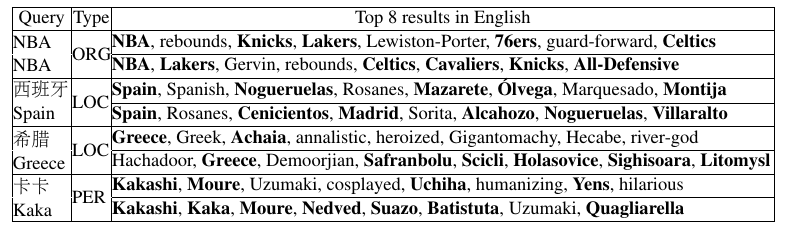
\includegraphics[height=3.5cm]{bwes.png}
\end{figure}
\end{frame}
\begin{frame}{Word embeddings. Обучение без разметки}
\textit{Rami Al-Rfou, Vivek Kulkarni, Bryan Perozzi, Steven Skiena.} POLYGLOT -NER: Massive Multilingual Named Entity Recognition, 2015.
\begin{itemize}
\item Разметка NE в 40 языках с использованием Word embeddings (совместная встречаемость слов в тексте), которые используются в качестве признаков при обучении.
\item Отсутствующие теги частей речи размечались методом точного соответствия.  
\item Оценка потерь. Оптимизация при помощи стохастического градиентного спуска. 
\end{itemize}
\end{frame}

\begin{frame}{PERSON}
\begin{figure}
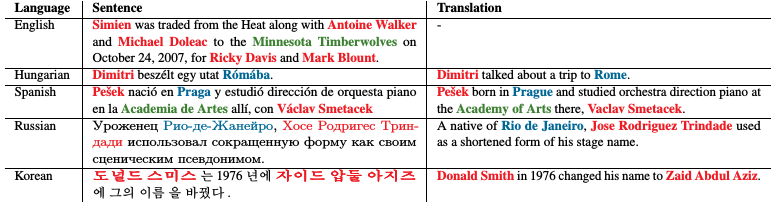
\includegraphics[height=3cm]{ner_em.png}
\end{figure}
\end{frame}

\begin{frame}{Ошибки. PER/ORG, LOC/ORG}
\begin{figure}
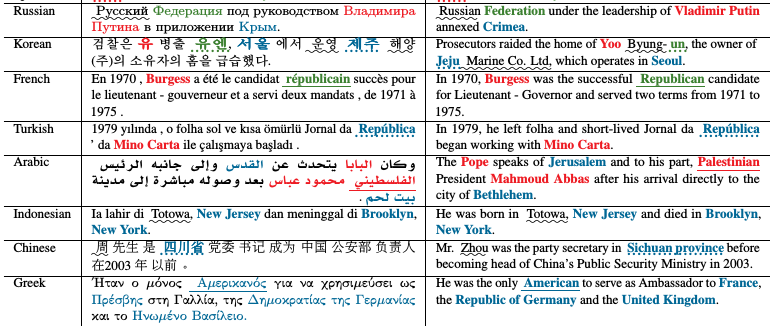
\includegraphics[height=5cm]{ner_err.png}
\end{figure}
\end{frame}

\begin{frame}{Оценка качества}
\begin{itemize}
\item Тексты CONLL для крупных языков.
\item Distant Evaluation при помощи машинного перевода. 
\end{itemize}
\end{frame}

\begin{frame}{Результаты}
\begin{figure}
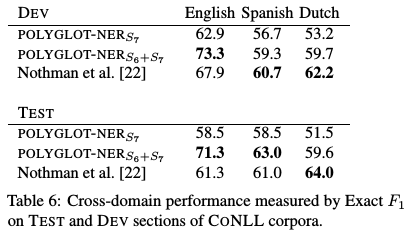
\includegraphics[height=6cm]{ner_conll_test.png}
\end{figure}
\end{frame}

\section{Readability}
\begin{frame}{Readability}

Readability — сумму всех элементов текстового материала, котоыре влияют на понимание текста, скорость прочтения и уровень интереса к материалу

\textbf{Основные методики}
\begin{itemize}
\item Подсчет соотношения длины предложений и количества слов (FRE, FKR);
\item Подсчет соотношения длины предложений и количества сложных слов (NDC)
\item Применение машинного обучения
\end{itemize}

\end{frame}

\begin{frame}{Automatic Text Simplification}

Horacio Saggion, 2017.
\textbf{Виды признаков для оценки ридабилити} 
\begin{itemize}
\item Лексико-семантические (словарные) признаки: относительная частота слов, оценка вида и кол-ва токенов, вероятностные лингвистические модели
\item Психолингвистические признаки: возраст понимания, конкретность, полисемия 
\item Синтаксические признаки — длина предложения, уровни в деревьях 
\item Дискурсивные признаки — кореерентные связи, именнованные сущности, плотность текста
\item Семантические и прагматические признаки: использование идиом, культурных отсылок и образов, тип текста (мнение, сатира и т.д.)
\end{itemize}
\end{frame}

\begin{frame}{A Multi-task Approach to Predict Likability of Books}

Suraj Maharjan, Manuel Montes-y-Gomez, Thamar Solorio, John Arevalo and Fabio A. Gonzalez
\textbf{Как оценить ридабилити художественного текста?} 
\begin{itemize}
\item Создали нейронную сеть и научили ее предсказывать потенциальную успешность книги
\item Использовали классические метрики и машинное обучение
\item Обучили 25 моделей
\item Наилучший результат — 71%
\item И его показала не нейросеть...
\end{itemize}
\end{frame}

\begin{frame}{Какие еще бывают исследования?}

\begin{itemize}
\item Изменение сложности научных текстов за последние 200 лет
\item Измерение ридабилити узкоспецаиилизрованных медицинских текстов
\item Измерение ридабилити текстов о финансах и юриспруденции

\end{itemize}
\end{frame}

\end{document}
